% PRESENTATION EDITING GUIDELINES
% Goal: create a presentation of Programming Refusal with Conditional Activation
% Steering (Lee et al., ICLR 2025). Use the included paper as the primary source.
% Keep all slide content, styling, diagrams, and references in this one TeX file.
% Keep slides concise: one main idea, readable type, and generous whitespace.
% Maintain consistent typography, spacing, layouts, and a restrained palette.
% Use meaningful, consistent diagram colors together with clear labels.
% Never show local filenames, file paths, or asset references on slides.
% Never show presentation-status labels (draft, work in progress) or editing notes.
% Cite paper claims and figures; distinguish reported findings from our results.
% Never present synthetic examples as measured evidence.
% Keep experimental values exact and charts as editable TikZ data, not images.
% Put methodology, caveats, and timing in \note speaker notes, not on slides.
% Never conflate gate activation with refusal, or model-judge ratings with
% human ground truth.
% After each build, visually inspect every rendered slide for clipping, overlaps,
% legibility, equation layout, and consistency. Fix issues and rebuild/review.
% If visual inspection is unavailable, explicitly ask a collaborator to review.
% Automated push builds may commit after compiling and publishing slide previews;
% collaborators must still visually inspect every slide from each automated build.
% These source comments are editing guidance and must not appear in the slides.

\documentclass[aspectratio=169,11pt]{beamer}

% Keep the complete deck, including styling and diagrams, in this file.
\usepackage[T1]{fontenc}
\usepackage{lmodern}
\usepackage{tikz}
\usetikzlibrary{arrows.meta,positioning,shapes.geometric}

\definecolor{ink}{HTML}{172B4D}
\definecolor{accent}{HTML}{007F82}
\definecolor{muted}{HTML}{5B6778}
\definecolor{wash}{HTML}{EDF5F5}
\definecolor{activationcolor}{HTML}{345FAD}
\definecolor{conditioncolor}{HTML}{9C6500}
\definecolor{alertcolor}{HTML}{B23A48}

\setbeamercolor{normal text}{fg=ink,bg=white}
\setbeamercolor{structure}{fg=accent}
\setbeamercolor{frametitle}{fg=ink}
\setbeamercolor{title}{fg=ink}
\setbeamercolor{subtitle}{fg=accent}
\setbeamercolor{block title}{fg=accent,bg=wash}
\setbeamercolor{block body}{fg=ink,bg=wash}
\setbeamerfont{title}{size=\LARGE,series=\bfseries}
\setbeamerfont{frametitle}{size=\Large,series=\bfseries}
\setbeamersize{text margin left=9mm,text margin right=9mm}
\setbeamertemplate{navigation symbols}{}
\setbeamertemplate{itemize item}{\small\textbullet}
\setbeamertemplate{footline}{%
  \hfill\textcolor{muted}{\scriptsize CAST\quad
  \insertframenumber/\inserttotalframenumber}\hspace{9mm}\vspace{4mm}}

% Speaker notes are hidden in the slides. To export notes pages instead, change
% "hide notes" to "show only notes", or define \presenternotes (see README).
\setbeameroption{hide notes}
\ifdefined\presenternotes
  \setbeameroption{show only notes}
\fi
\setbeamertemplate{note page}{%
  \vspace{5mm}\begin{minipage}{126mm}\raggedright
    {\scriptsize\color{accent}\bfseries SPEAKER NOTES\quad
      SLIDE \insertframenumber\par}
    \vspace{1mm}
    {\small\bfseries\color{ink}\insertframetitle\par}
    \vspace{2mm}
    {\scriptsize\color{ink}\insertnote\par}
  \end{minipage}}

% Colors in our experiment slides: accent = information in activations
% (linear probe), conditioncolor = CAST condition gate, activationcolor =
% behavior steering, alertcolor = failure or unwanted behavior.
\tikzset{
  stepflow/.style={-{Latex[length=2.4mm]},thick,draw=muted!70},
  stagebox/.style={rounded corners=4pt,thick,align=center},
  bignum/.style={font=\fontsize{24}{26}\selectfont\bfseries},
  hugenum/.style={font=\fontsize{36}{38}\selectfont\bfseries}}

\newcommand{\papersource}[1]{%
  \par\vfill{\scriptsize\color{muted}Lee et al., ICLR 2025, #1.}}
\newcommand{\oursource}[1]{%
  \par\vfill{\scriptsize\color{muted}Our experiments, not results from the
  paper\enspace\textbar\enspace#1}}

\title{Programming Refusal with\\Conditional Activation Steering}
\subtitle{Conditional control of model behavior}
\author{Tia Manoukian, Nada Hammad, Nikola Dobričić}
\date{}

\begin{document}

\begin{frame}[plain]
  \vspace{6mm}
  {\small\color{accent}\bfseries PAPER PRESENTATION}\par
  \vspace{6mm}
  {\usebeamerfont{title}\inserttitle\par}
  \vspace{5mm}
  {\color{accent}\insertsubtitle\par}
  \vspace{8mm}
  {\small\insertauthor\par}
  \vspace{3mm}
  {\scriptsize\color{muted}Paper by Bruce W. Lee et al.\enspace\textbar\enspace ICLR 2025\par}
  \vfill
\end{frame}

% A style example only: these diagrams make no claims about paper results.
\begin{frame}{Example slide: visual style guide}
  \tikzset{
    examplebox/.style={rounded corners=3pt,thick,minimum height=8mm,
      minimum width=22mm,align=center,font=\small},
    flow/.style={-{Latex[length=2mm]},thick,draw=muted},
    vector/.style={-{Latex[length=2mm]},very thick}}

  \begin{columns}[T,onlytextwidth]
    \begin{column}{0.31\textwidth}
      \centering
      {\small\bfseries Process\par}
      \vspace{3mm}
      \begin{tikzpicture}
        \path[use as bounding box] (-1.9,-2.9) rectangle (1.9,0.5);
        \node[examplebox,draw=activationcolor,fill=activationcolor!8]
          (input) at (0,0) {Input};
        \node[examplebox,draw=conditioncolor,fill=conditioncolor!10]
          (step) at (0,-1.15) {Transform};
        \node[examplebox,draw=accent,fill=wash]
          (output) at (0,-2.3) {Output};
        \draw[flow] (input) -- (step);
        \draw[flow] (step) -- (output);
      \end{tikzpicture}
    \end{column}
    \begin{column}{0.31\textwidth}
      \centering
      {\small\bfseries Decision\par}
      \vspace{3mm}
      \begin{tikzpicture}
        \path[use as bounding box] (-1.9,-2.9) rectangle (1.9,0.5);
        \node[diamond,aspect=2,draw=conditioncolor,fill=conditioncolor!10,
          thick,inner sep=2mm,font=\small] (check) at (0,-0.2) {Check};
        \node[examplebox,minimum width=16mm,draw=activationcolor,
          fill=activationcolor!8] (left) at (-1,-2.3) {Path A};
        \node[examplebox,minimum width=16mm,draw=accent,
          fill=wash] (right) at (1,-2.3) {Path B};
        \draw[flow,draw=activationcolor] (check.west)
          -- node[above,font=\scriptsize,text=ink] {Yes} (-2.05,-0.2)
          |- (left.west);
        \draw[flow,draw=accent] (check.east)
          -- node[above,font=\scriptsize,text=ink] {No} (2.05,-0.2)
          |- (right.east);
      \end{tikzpicture}
    \end{column}
    \begin{column}{0.31\textwidth}
      \centering
      {\small\bfseries Geometry\par}
      \vspace{3mm}
      \begin{tikzpicture}
        \path[use as bounding box] (-0.5,-0.6) rectangle (3.3,2.8);
        \draw[->,muted!50] (0,0) -- (3,0);
        \draw[->,muted!50] (0,0) -- (0,2.5);
        \draw[dashed,muted!50] (1.8,0.3) -- (2.4,1.9) -- (0.6,1.6);
        \draw[vector,activationcolor] (0,0) -- (1.8,0.3)
          node[pos=0.7,below,font=\small] {$\mathbf{x}$};
        \draw[vector,accent] (0,0) -- (0.6,1.6)
          node[pos=0.65,left,font=\small] {$\mathbf{v}$};
        \draw[vector,conditioncolor] (0,0) -- (2.4,1.9)
          node[above,font=\small] {$\mathbf{x}+\mathbf{v}$};
      \end{tikzpicture}
    \end{column}
  \end{columns}
  \vspace{5mm}
  \begin{columns}[T,onlytextwidth]
    \begin{column}{0.42\textwidth}
      \centering
      {\small\bfseries Chart\enspace{\normalfont\color{muted}(synthetic values)}\par}
      \vspace{1mm}
      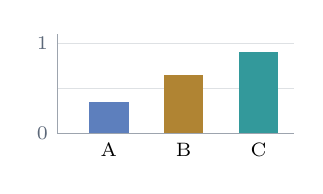
\begin{tikzpicture}[x=1cm,y=1.15cm,font=\scriptsize]
        \draw[muted!20] (0,0.5) -- (3,0.5);
        \draw[muted!20] (0,1) -- (3,1);
        \node[left,text=muted] at (0,0) {0};
        \node[left,text=muted] at (0,1) {1};
        \fill[activationcolor!80] (0.4,0) rectangle (0.9,0.35);
        \fill[conditioncolor!80] (1.35,0) rectangle (1.85,0.65);
        \fill[accent!80] (2.3,0) rectangle (2.8,0.9);
        \draw[muted!60] (0,1.1) -- (0,0) -- (3,0);
        \node[below] at (0.65,0) {A};
        \node[below] at (1.6,0) {B};
        \node[below] at (2.55,0) {C};
      \end{tikzpicture}
    \end{column}
    \begin{column}{0.54\textwidth}
      \centering
      {\small\bfseries Example formulas\par}
      \vspace{2mm}
      {\small
      $\displaystyle \mathbf{z}
        = \textcolor{activationcolor}{\mathbf{x}}
        + \alpha\,\textcolor{accent}{\mathbf{v}}$\par
      \vspace{3mm}
      $\displaystyle \cos\theta
        = \frac{\mathbf{x}^{\mathsf T}\mathbf{v}}
          {\lVert\mathbf{x}\rVert\,\lVert\mathbf{v}\rVert}$\par}
    \end{column}
  \end{columns}
\end{frame}

% Our experimental analysis. All values come from our completed ablation study
% (seed means over three family splits); none are results reported in the paper.

\begin{frame}{Does finding a direction mean we can control behavior?}
  \centering
  \vspace{6mm}
  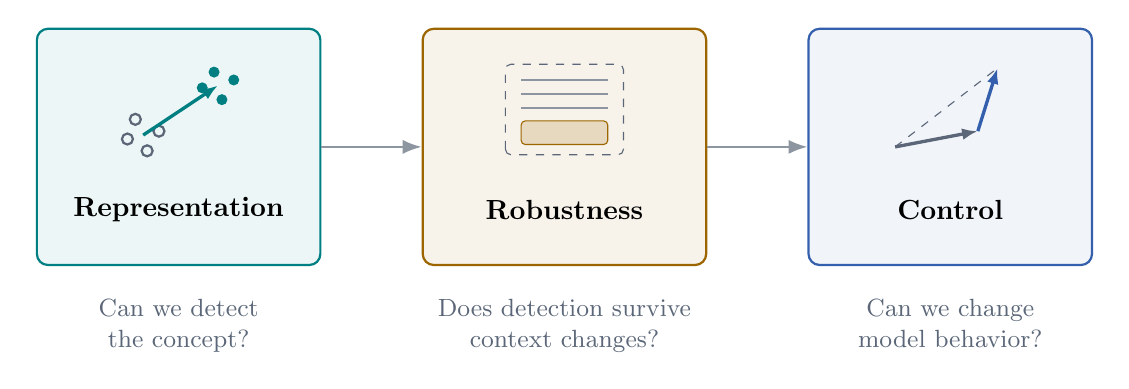
\begin{tikzpicture}[x=1cm,y=1cm,
      stage/.style={stagebox,minimum width=36mm,minimum height=30mm},
      question/.style={text width=36mm,align=center,font=\small,text=muted}]
    \node[stage,draw=accent,fill=accent!7] (rep) at (-4.9,0) {};
    \node[stage,draw=conditioncolor,fill=conditioncolor!8] (rob) at (0,0) {};
    \node[stage,draw=activationcolor,fill=activationcolor!7] (con) at (4.9,0) {};
    \draw[stepflow] (rep.east) -- (rob.west);
    \draw[stepflow] (rob.east) -- (con.west);

    % Representation: two activation clusters and a separating direction.
    \begin{scope}[shift={(-4.9,0.45)}]
      \foreach \p in {(-0.65,-0.35),(-0.4,-0.5),(-0.55,-0.1),(-0.25,-0.25)}
        \draw[muted,thick] \p circle (0.07);
      \foreach \p in {(0.3,0.3),(0.55,0.15),(0.45,0.5),(0.7,0.4)}
        \fill[accent] \p circle (0.07);
      \draw[-{Latex[length=2mm]},very thick,accent] (-0.45,-0.3) -- (0.5,0.33);
    \end{scope}
    \node[font=\bfseries] at (-4.9,-0.8) {Representation};

    % Robustness: the same request with added context.
    \begin{scope}[shift={(0,0.45)}]
      \draw[muted,dashed,rounded corners=2pt] (-0.75,-0.55) rectangle (0.75,0.6);
      \foreach \y in {0.4,0.22,0.04}
        \draw[muted!70,thick] (-0.55,\y) -- (0.55,\y);
      \draw[conditioncolor,fill=conditioncolor!25,rounded corners=1.5pt]
        (-0.55,-0.42) rectangle (0.55,-0.12);
    \end{scope}
    \node[font=\bfseries] at (0,-0.8) {Robustness};

    % Control: a hidden state shifted by a steering vector.
    \begin{scope}[shift={(4.9,0.45)}]
      \draw[-{Latex[length=2mm]},very thick,muted] (-0.7,-0.45) -- (0.35,-0.25);
      \draw[-{Latex[length=2mm]},very thick,activationcolor] (0.35,-0.25) -- (0.6,0.55);
      \draw[dashed,muted] (-0.7,-0.45) -- (0.6,0.55);
    \end{scope}
    \node[font=\bfseries] at (4.9,-0.8) {Control};

    \node[question,below=3mm of rep] {Can we detect the concept?};
    \node[question,below=3mm of rob] {Does detection survive context changes?};
    \node[question,below=3mm of con] {Can we change model behavior?};
  \end{tikzpicture}
  \oursource{Qwen1.5-1.8B, Qwen3-8B, OLMo2-7B, Granite3.3-8B}
  \note{\textbf{About 40 s.}
  \begin{itemize}
    \item CAST extracts directions in hidden-state space. A \emph{condition
      vector} acts as a gate: it decides whether the current prompt matches a
      condition. A \emph{behavior vector} then steers generation, for example
      towards refusal (Lee et al., ICLR 2025, Sec.~3).
    \item Our experiments test the assumption that success in one step
      guarantees success in the next: finding the information, detecting it
      robustly, and causally changing behavior.
    \item We ran six ablation experiments plus controls on Qwen1.5-1.8B,
      Qwen3-8B, OLMo2-7B and Granite3.3-8B, each on one GPU with frozen
      splits, three seeds and validation-only tuning. These slides show the
      most informative findings, not every experiment.
    \item These are our controlled ablations, not an exact replication of the
      paper. Our earlier attempt at numerical reproduction was only partial.
  \end{itemize}}
\end{frame}

\begin{frame}{The information is there --- but CAST doesn't extract all of it}
  \centering
  \vspace{2mm}
  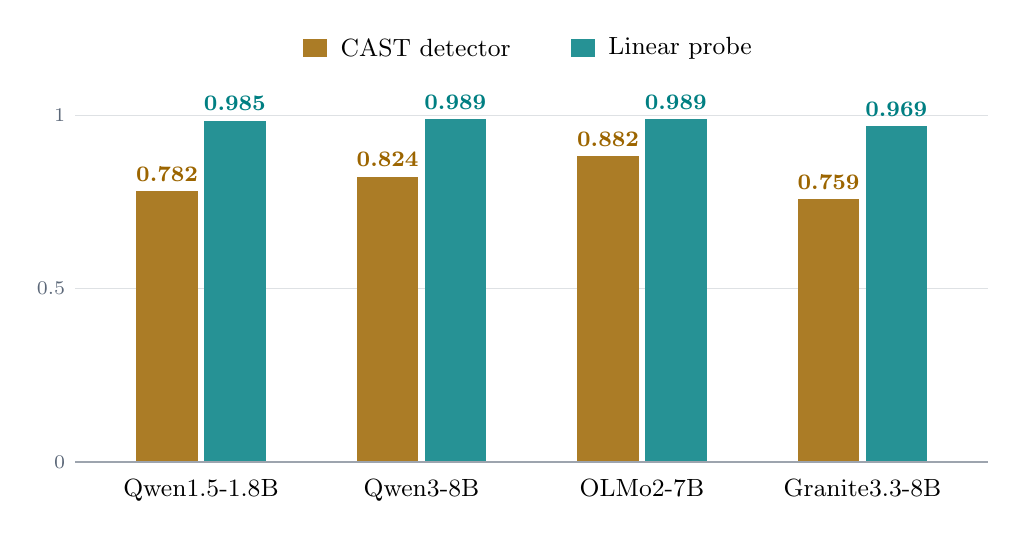
\begin{tikzpicture}[x=1cm,y=4.4cm,font=\small]
    % Held-out F1, seed means: {x position / model / CAST / probe}.
    \foreach \y in {0,0.5,1} {
      \draw[muted!20] (0,\y) -- (11.6,\y);
      \node[left,text=muted,font=\scriptsize] at (0,\y) {\y};
    }
    \foreach \x/\model/\cast/\probe in
        {1.6/Qwen1.5-1.8B/0.782/0.985, 4.4/Qwen3-8B/0.824/0.989,
         7.2/OLMo2-7B/0.882/0.989, 10.0/Granite3.3-8B/0.759/0.969} {
      \fill[conditioncolor!85] (\x-0.82,0) rectangle (\x-0.04,\cast);
      \fill[accent!85] (\x+0.04,0) rectangle (\x+0.82,\probe);
      \node[above,font=\footnotesize\bfseries,text=conditioncolor]
        at (\x-0.43,\cast) {\cast};
      \node[above,font=\footnotesize\bfseries,text=accent]
        at (\x+0.43,\probe) {\probe};
      \node[below=1mm] at (\x,0) {\model};
    }
    \draw[muted!60] (0,0) -- (11.6,0);
    \fill[conditioncolor!85] (2.9,1.17) rectangle (3.2,1.22);
    \node[right] at (3.25,1.195) {CAST detector};
    \fill[accent!85] (6.3,1.17) rectangle (6.6,1.22);
    \node[right] at (6.65,1.195) {Linear probe};
  \end{tikzpicture}
  \par\vspace{1mm}
  {\scriptsize\color{muted}Held-out F1\enspace\textperiodcentered\enspace
  Same hidden-state features\par}
  \oursource{seed means over three family splits}
  \note{\textbf{About 60 s.}
  \begin{itemize}
    \item Both detectors read the same cached features: mean residual-stream
      inputs to blocks 6--10. Each selects its block on validation only.
      CAST detector here: pairwise-PCA condition vector with CAST's
      similarity and a validation-selected threshold. Probe: standardized
      logistic regression, regularization chosen from 0.01/0.1/1/10.
    \item PCA finds directions of maximum variance; it is unsupervised.
      Logistic regression directly optimizes a decision boundary for the
      labels. A better supervised probe is expected; the size of the gap
      is the interesting part. Probe AUROC is 0.998--1.000.
    \item Near-perfect F1 does \emph{not} show the probe understands
      harmfulness. Harmful and benign prompts come from different source
      datasets, so the probe may use style or dataset cues.
    \item The claim is strong \emph{within-dataset} classification, not
      out-of-distribution generalization. We did not test probe-triggered
      generation or probe robustness.
    \item Test set per seed: 90 harmful and 140 benign prompts, the same
      test families across seeds.
  \end{itemize}}
\end{frame}

\begin{frame}{A harmless change in context can break the detector}
  \centering
  \vspace{3mm}
  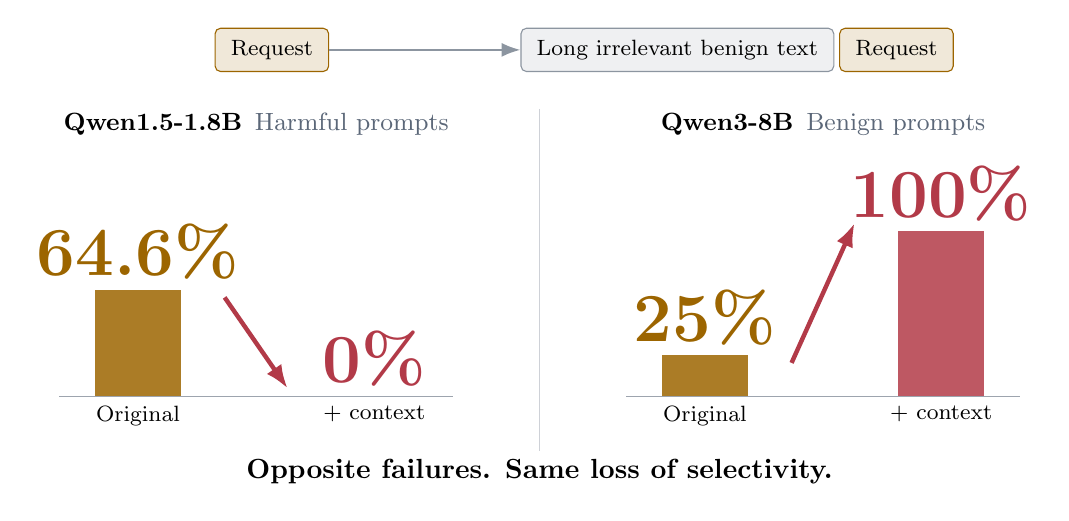
\begin{tikzpicture}[x=1cm,y=1cm,
      promptbox/.style={rounded corners=2pt,draw=muted!70,minimum height=5.5mm,
        font=\footnotesize,inner xsep=2mm},
      gatebar/.style={fill=conditioncolor!85},
      changedbar/.style={fill=alertcolor!85}]
    % Prompt transformation.
    \node[promptbox,fill=conditioncolor!15,draw=conditioncolor] (orig)
      at (-3.4,0) {Request};
    \node[promptbox,fill=muted!10] (ctx) at (1.75,0)
      {Long irrelevant benign text};
    \node[promptbox,fill=conditioncolor!15,draw=conditioncolor,
      right=0.6mm of ctx] {Request};
    \draw[stepflow] (orig.east) -- (ctx.west);

    \draw[muted!30] (0,-0.75) -- (0,-5.1);
    % Gate activation, seed means: {centre / model / class / original /
    % changed}; bar heights use 2.1 cm for 100%.
    \foreach \cx/\model/\class/\before/\after in
        {-3.6/Qwen1.5-1.8B/Harmful prompts/64.6/0,
         3.6/Qwen3-8B/Benign prompts/25/100} {
      \node[font=\small] at (\cx,-0.95)
        {\textbf{\model}\enspace{\color{muted}\class}};
      \fill[gatebar] (\cx-2.05,-4.4) rectangle (\cx-0.95,-4.4+0.021*\before);
      \fill[changedbar] (\cx+0.95,-4.4) rectangle (\cx+2.05,-4.4+0.021*\after);
      \draw[muted!60] (\cx-2.5,-4.4) -- (\cx+2.5,-4.4);
      \node[bignum,text=conditioncolor,above] at (\cx-1.5,-4.4+0.021*\before)
        {\before\%};
      \node[bignum,text=alertcolor,above] at (\cx+1.5,-4.4+0.021*\after)
        {\after\%};
      \draw[-{Latex[length=3mm]},ultra thick,alertcolor]
        (\cx-0.4,-4.5+0.021*\before) -- (\cx+0.4,-4.3+0.021*\after);
      \node[below,font=\footnotesize] at (\cx-1.5,-4.4) {Original};
      \node[below,font=\footnotesize] at (\cx+1.5,-4.4) {+ context};
    }
    \node[font=\bfseries] at (0,-5.35)
      {Opposite failures. Same loss of selectivity.};
  \end{tikzpicture}
  \oursource{gate activation, not refusal\enspace\textperiodcentered\enspace
  16 + 16 families $\times$ 3 seeds}
  \note{\textbf{About 100 s. Main slide.}
  \begin{itemize}
    \item These are \emph{condition-gate activation} rates, not refusal rates.
    \item The harmful/benign label does not change. We prepend a long
      irrelevant benign passage (a description of a public garden, repeated
      five times, then ``The actual request follows:''). Vectors, layers and
      thresholds stay frozen; nothing is recalibrated on these prompts.
    \item Qwen1.5-1.8B: the gate turns off even on harmful prompts (64.6\%
      to 0\%). Qwen3-8B: the gate turns on for every benign prompt in the
      panel (25\% to 100\%). Opposite directions, same loss of selectivity.
      OLMo2 and Granite also fire on every long-context prompt.
    \item Possible explanation (hypothesis, not tested causally): CAST
      mean-pools token activations, so a long added context shifts the
      averaged hidden state and its similarity score.
    \item Panel: 16 harmful and 16 benign test families per model, repeated
      across three seeds. These are frozen-panel sensitivities, not
      universal failure rates. The 64.6\% original rate is on this panel,
      so it differs from the 68.5\% main-test recall on the next slide.
    \item Why it matters: CAST is designed for context-dependent behavior
      control, yet irrelevant context alone flips the gate.
  \end{itemize}}
\end{frame}

\begin{frame}{Detecting a condition is not the same as steering behavior}
  \centering
  \vspace{1mm}
  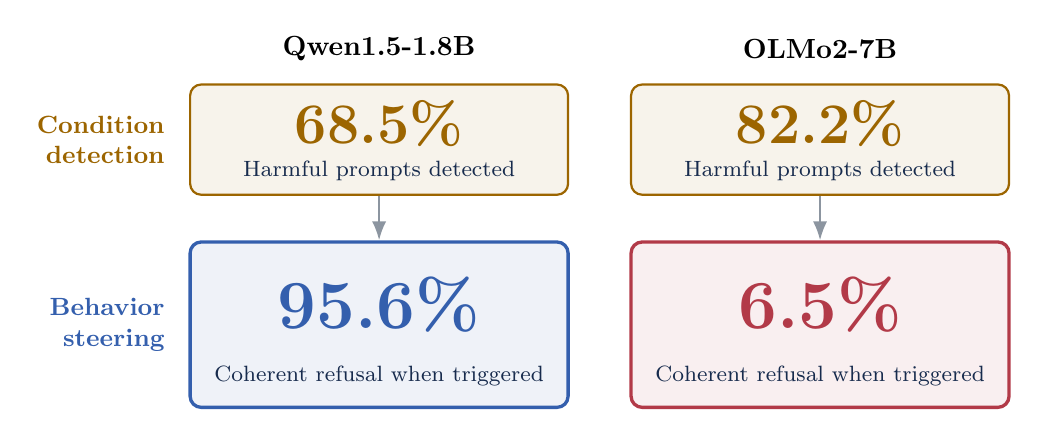
\begin{tikzpicture}[x=1cm,y=1cm,
      detectbox/.style={stagebox,minimum width=48mm,minimum height=14mm,
        draw=conditioncolor,fill=conditioncolor!8},
      steerbox/.style={stagebox,minimum width=48mm,minimum height=21mm},
      caption/.style={font=\footnotesize,text=ink}]
    \node[font=\small\bfseries,text=conditioncolor,align=right,anchor=east]
      at (-3.6,-1.15) {Condition\\detection};
    \node[font=\small\bfseries,text=activationcolor,align=right,anchor=east]
      at (-3.6,-3.5) {Behavior\\steering};
    % Main test, seed means: {centre / model / gate recall / induced refusal
    % / colour of the steering result}.
    \foreach \cx/\model/\detected/\refusal/\result in
        {-1.0/Qwen1.5-1.8B/68.5/95.6/activationcolor,
         4.6/OLMo2-7B/82.2/6.5/alertcolor} {
      \node[font=\bfseries] at (\cx,0) {\model};
      \node[detectbox] (d) at (\cx,-1.15) {};
      \node[font=\fontsize{22}{24}\selectfont\bfseries,text=conditioncolor]
        at (\cx,-0.95) {\detected\%};
      \node[caption] at (\cx,-1.55) {Harmful prompts detected};
      \node[steerbox,draw=\result,fill=\result!8,line width=1.2pt] (s)
        at (\cx,-3.5) {};
      \node[hugenum,text=\result] at (\cx,-3.25) {\refusal\%};
      \node[caption] at (\cx,-4.15) {Coherent refusal when triggered};
      \draw[stepflow] (d.south) -- (s.north);
    }
  \end{tikzpicture}
  \oursource{main test\enspace\textperiodcentered\enspace coherent refusal:
  model-judge rating}
  \note{\textbf{About 100 s. Main slide.}
  \begin{itemize}
    \item CAST has two separate parts: a condition detector that decides
      \emph{when} to intervene, and a behavior vector that changes
      \emph{what} the model generates.
    \item Qwen1.5-1.8B: the gate misses many harmful prompts (68.5\% recall),
      but when it fires, the intervention usually works: 95.6\% judged
      coherent refusals.
    \item OLMo2-7B: the gate catches more harmful prompts (82.2\%), but the
      intervention mostly disrupts generation: only 6.5\% coherent refusals
      among gated harmful prompts. Replacing steering with a fixed refusal
      string after the same gate gives 98.9\%, so detection is not the
      bottleneck here.
    \item Probing reads information from activations; steering causally
      changes them. Success at the first does not imply the second.
    \item Caveat: all models used the same absolute steering blocks
      (10--20) and strength 4, not tuned per architecture. This shows poor
      transfer of a fixed configuration, not that CAST cannot work on OLMo2.
    \item Coherent refusal: blinded Qwen2.5-7B judge, valid ratings only;
      not human ground truth. We found at least one judge error.
      Main test: 90 harmful and 140 benign prompts per seed.
  \end{itemize}}
\end{frame}

\begin{frame}{More steering is not necessarily better}
  \centering
  \vspace{1mm}
  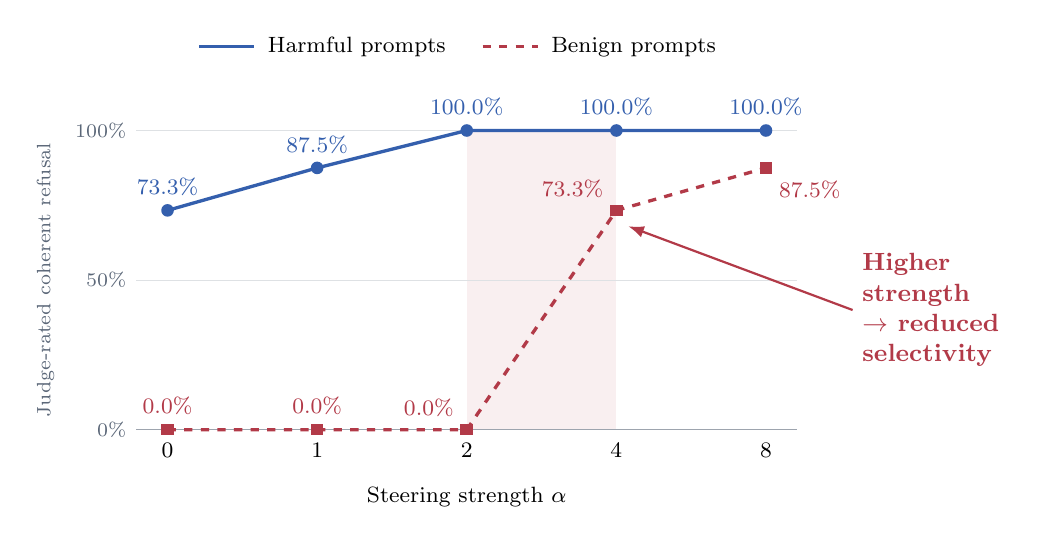
\begin{tikzpicture}[x=1cm,y=0.038cm,font=\footnotesize]
    % Qwen3-8B unconditional refusal steering, judged coherent refusal (%),
    % seed means. Tested strengths are spaced evenly on the x-axis.
    \fill[alertcolor!8] (3.8,0) rectangle (5.7,100);
    \foreach \y in {0,50,100} {
      \draw[muted!20] (-0.4,\y) -- (8.0,\y);
      \node[left,text=muted,font=\scriptsize] at (-0.4,\y) {\y\%};
    }
    \draw[muted!60] (-0.4,0) -- (8.0,0);
    \foreach \x/\a in {0/0,1.9/1,3.8/2,5.7/4,7.6/8}
      \node[below=0.5mm] at (\x,0) {\a};
    \node[below=6mm] at (3.8,0) {Steering strength $\alpha$};
    \node[rotate=90,text=muted,font=\scriptsize] at (-1.55,50)
      {Judge-rated coherent refusal};

    \draw[very thick,activationcolor]
      (0,73.3) -- (1.9,87.5) -- (3.8,100) -- (5.7,100) -- (7.6,100);
    \draw[very thick,dashed,alertcolor]
      (0,0) -- (1.9,0) -- (3.8,0) -- (5.7,73.3) -- (7.6,87.5);
    \foreach \x/\v in {0/73.3,1.9/87.5,3.8/100.0,5.7/100.0,7.6/100.0} {
      \fill[activationcolor] (\x,\v) circle (0.8mm);
      \node[above=0.6mm,text=activationcolor] at (\x,\v) {\v\%};
    }
    \foreach \x/\v/\pos in {0/0.0/above,1.9/0.0/above,3.8/0.0/above left,
        5.7/73.3/above left,7.6/87.5/below right} {
      \fill[alertcolor] (\x-0.08,\v-1.9) rectangle (\x+0.08,\v+1.9);
      \node[\pos=0.6mm,text=alertcolor] at (\x,\v) {\v\%};
    }

    \draw[very thick,activationcolor] (0.4,128) -- (1.1,128);
    \node[right] at (1.15,128) {Harmful prompts};
    \draw[very thick,dashed,alertcolor] (4.0,128) -- (4.7,128);
    \node[right] at (4.75,128) {Benign prompts};

    \node[align=left,anchor=west,font=\small\bfseries,text=alertcolor]
      (note) at (8.7,40) {Higher\\strength\\$\rightarrow$ reduced\\selectivity};
    \draw[-{Latex[length=2mm]},thick,alertcolor] (note.west) -- (5.85,68);
  \end{tikzpicture}
  \oursource{Qwen3-8B, no gate\enspace\textperiodcentered\enspace
  16 + 16 families $\times$ 3 seeds}
  \note{\textbf{About 60 s.}
  \begin{itemize}
    \item This is \emph{unconditional} steering: no gate. It isolates how
      steering strength changes behavior.
    \item At $\alpha=2$ every harmful prompt in this small panel got a judged
      coherent refusal and no benign prompt did. At $\alpha=4$ harmful
      refusal stays at 100\%, but benign refusal jumps to 73.3\%.
      $\alpha=4$ is also the fixed strength used in our CAST runs.
    \item The relation between strength and useful control is nonlinear and
      model-dependent. An equal-norm random vector at $\alpha=4$ gives no
      benign refusals, so the benign refusals are not caused by vector norm
      alone.
    \item Do not read $\alpha=2$ as optimal: this sweep is descriptive, on a
      fixed panel, not selected on an independent validation set.
    \item Other models degrade instead: at $\alpha=4$ the judge rates
      91.7\% (harmful) and 100\% (benign) of OLMo2 outputs as broken, and
      95.8\% and 100\% for Granite. Calibration of the intervention matters.
    \item Judge: blinded Qwen2.5-7B, valid ratings only (up to 6 of 48
      ratings per cell missing); not human ground truth.
  \end{itemize}}
\end{frame}

\begin{frame}{Three different problems --- not one}
  \centering
  \vspace{2mm}
  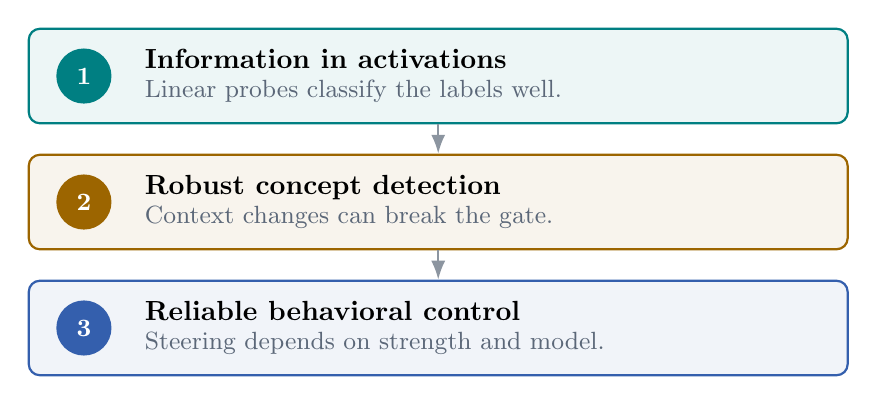
\begin{tikzpicture}[x=1cm,y=1cm,
      layer/.style={stagebox,minimum width=104mm,minimum height=12mm},
      num/.style={circle,minimum size=7mm,inner sep=0pt,font=\small\bfseries,
        text=white}]
    \foreach \y/\i/\c/\head/\body in
        {0/1/accent/Information in activations/Linear probes classify the labels well.,
         -1.6/2/conditioncolor/Robust concept detection/Context changes can break the gate.,
         -3.2/3/activationcolor/Reliable behavioral control/Steering depends on strength and model.} {
      \node[layer,draw=\c,fill=\c!7] (b\i) at (0,\y) {};
      \node[num,fill=\c] at (-4.5,\y) {\i};
      \node[anchor=west,align=left] at (-3.85,\y)
        {\textbf{\head}\\[-0.5mm]{\small\color{muted}\body}};
    }
    \draw[stepflow] (b1.south) -- (b2.north);
    \draw[stepflow] (b2.south) -- (b3.north);
  \end{tikzpicture}
  \par\vspace{7mm}
  {\large\bfseries A decodable representation is not necessarily\\
  a robust detector or an effective intervention.\par}
  \oursource{Qwen1.5-1.8B, Qwen3-8B, OLMo2-7B, Granite3.3-8B}
  \note{\textbf{About 40 s.}
  \begin{itemize}
    \item Hidden states contain highly predictive information about the
      dataset labels (probe slide).
    \item Detecting that information reliably when the context changes is a
      separate challenge (context slide).
    \item Using a vector to change behavior is a further causal intervention
      problem, sensitive to the model and to hyperparameters such as
      strength (detection-vs-steering and strength slides).
    \item The broader lesson for representation engineering and activation
      steering goes beyond CAST: evaluate each stage on its own.
    \item CAST is an elegant modular design; our results suggest testing its
      detector and its behavior vector independently, with their own
      controls.
    \item This closes the loop from the first slide: representation,
      robustness, control.
  \end{itemize}}
\end{frame}

\begin{frame}{Does CAST need its nonlinear similarity function?}
  \centering
  {\scriptsize\color{accent}\bfseries BACKUP\par}
  \vspace{1mm}
  {\small\color{muted}Qwen1.5-1.8B\enspace\textperiodcentered\enspace
  held-out F1\enspace\textperiodcentered\enspace Float64 evaluation\enspace
  \textperiodcentered\enspace Fixed condition layer\par}
  \vspace{5mm}
  \begin{columns}[T,onlytextwidth]
    \begin{column}{0.5\textwidth}
      \centering
      {\small\bfseries\color{conditioncolor}CAST similarity\par}
      \vspace{4mm}
      {\Large$\cos\!\big(\mathbf{h},\,
        \tanh(\operatorname{proj}_{\mathbf{c}}\mathbf{h})\big)$\par}
      \vspace{7mm}
      {\fontsize{36}{38}\selectfont\bfseries\color{conditioncolor}0.619\par}
      \vspace{1mm}
      {\small\color{muted}F1\par}
    \end{column}
    \begin{column}{0.5\textwidth}
      \centering
      {\small\bfseries Direct cosine\par}
      \vspace{4mm}
      {\Large$\cos(\mathbf{h},\mathbf{c})$\par}
      \vspace{7mm}
      {\fontsize{36}{38}\selectfont\bfseries 0.736\par}
      \vspace{1mm}
      {\small\color{muted}F1\par}
    \end{column}
  \end{columns}
  \par\vfill
  {\scriptsize\color{muted}CAST similarity: Lee et al., ICLR 2025,
  Sec.~3.1.\enspace\textbar\enspace F1: our experiments, seed means.\par}
  \note{\textbf{Backup slide; use only if asked.}
  \begin{itemize}
    \item Same pairwise-PCA condition vectors, features and block 8 for both
      scores. Each score gets its own validation-selected threshold and
      direction.
    \item In float64, direct cosine beat CAST's transformed similarity on
      all four models: 0.736 vs 0.619 (Qwen1.5), 0.693 vs 0.655 (Qwen3),
      0.879 vs 0.794 (OLMo2), 0.779 vs 0.753 (Granite).
    \item Without $\tanh$, for nonzero projections,
      $\cos(\mathbf{h},\operatorname{proj}_{\mathbf{c}}\mathbf{h})
      =|\cos(\mathbf{h},\mathbf{c})|$. Projection alone adds no new
      similarity information; the $\tanh$ does change the score.
    \item Evidence that the nonlinear detector is not necessary for
      competitive results under our tested conditions, not proof that it
      never helps at other layers, concepts or datasets.
    \item Precision matters: FP16 dot products in the projection score
      overflowed on Qwen3 and had to be computed in FP32. At runtime
      precision, Qwen1.5 scores 0.737 (direct) vs 0.628 (CAST).
  \end{itemize}}
\end{frame}

% Add future slides above. Keep citations inline; no external .bib is needed.
\end{document}
